\documentclass[aspectratio=169,11pt]{beamer}

% Shared style (ib-tutorials.sty at the repo root).
\makeatletter\def\input@path{{./}{../}}\makeatother
\usepackage{ib-tutorials}

\usepackage[utf8]{inputenc}
\usepackage{amsmath,amssymb}
\usepackage{booktabs}
\usepackage{array}
\newcolumntype{L}[1]{>{\raggedright\arraybackslash}p{#1}}
\usepackage{graphicx}
\graphicspath{{../pictures/4-ibfe/}{pictures/4-ibfe/}}
\usepackage{xcolor}
\usepackage{listings}
\usepackage{tikz}
\usetikzlibrary{arrows.meta,positioning,shapes.geometric,fit,calc,decorations.pathmorphing}
\usepackage{hyperref}

\newcommand{\sourcecredit}[1]{\vfill\begin{flushright}\tiny\textcolor{DarkGray}{#1}\end{flushright}}

\lstset{
  basicstyle=\ttfamily\scriptsize\color{BlackGray},
  keywordstyle=\color{NavyBlue}\bfseries,
  commentstyle=\color{DarkGray}\itshape,
  stringstyle=\color{OliveGreen},
  showstringspaces=false,
  columns=fullflexible,
  keepspaces=true,
  breaklines=true,
  breakindent=1em,
  frame=single,
  framerule=0.4pt,
  rulecolor=\color{LightGray},
  backgroundcolor=\color{LightGray!30},
  xleftmargin=0.25em,
  xrightmargin=0.25em
}
\lstdefinestyle{shell}{morecomment=[l]{\#}}
\lstdefinestyle{input}{morecomment=[l]{//}}
\lstdefinestyle{matlab}{morecomment=[l]{\%}}
\lstdefinestyle{python}{morecomment=[l]{\#}}
\lstdefinestyle{data}{}
\lstdefinestyle{tiny}{basicstyle=\ttfamily\tiny\color{BlackGray}}
\lstdefinestyle{inputtiny}{morecomment=[l]{//},basicstyle=\ttfamily\tiny\color{BlackGray}}
\lstdefinestyle{cpp}{language=C++,morecomment=[l]{//}}
\lstdefinestyle{cpptiny}{language=C++,morecomment=[l]{//},basicstyle=\ttfamily\tiny\color{BlackGray}}

\title[PK1 stress functions and body forces]{PK1 stress functions and body forces}
\subtitle{What IBAMR does with the first Piola--Kirchhoff stress, the neo-Hookean model in two parts, the other material laws in the examples, body and surface forces, and what the shear modulus and the tether stiffness do to the plate}
\author[Miller]{Laura A. Miller}
\institute[UArizona]{Department of Mathematics, University of Arizona}
\date{Using IB Software \textbullet\ Part IV \textbullet\ Chapter 19}

\begin{document}

% 1
\begin{frame}[plain]
\maketutorialtitlepanel{%
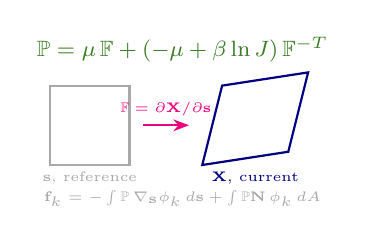
\begin{tikzpicture}[scale=0.84]
  % reference square and deformed parallelogram
  \draw[DarkGray,thick] (0.3,0.4) rectangle (1.5,1.6);
  \node[font=\tiny,text=DarkGray] at (0.9,0.2) {$\mathbf{s}$, reference};
  \draw[-{Stealth[length=2mm]},RubineRed,thick] (1.7,1.0) -- (2.4,1.0);
  \node[font=\tiny,text=RubineRed] at (2.05,1.25) {$\mathbb{F} = \partial\mathbf{X}/\partial\mathbf{s}$};
  \draw[NavyBlue,thick] (2.6,0.4) -- (3.9,0.6) -- (4.2,1.8) -- (2.9,1.6) -- cycle;
  \node[font=\tiny,text=NavyBlue] at (3.4,0.2) {$\mathbf{X}$, current};
  \node[font=\footnotesize,text=OliveGreen] at (2.3,2.15) {$\mathbb{P} = \mu\,\mathbb{F} + (-\mu + \beta\ln J)\,\mathbb{F}^{-T}$};
  \node[font=\tiny,text=DarkGray] at (2.3,-0.1) {$\mathbf{f}_k = -\int \mathbb{P}\,\nabla_{\mathbf{s}}\phi_k\,d\mathbf{s} + \int \mathbb{P}\mathbf{N}\,\phi_k\,dA$};
\end{tikzpicture}}
\end{frame}

% 2
\begin{frame}{Learning goals}
\label{fr:goals}
\scriptsize By the end of this chapter you should be able to:
\begin{enumerate}
  \item name the four quantities a stress function sees ($\mathbf{s}$, $\mathbf{X}$, $\mathbb{F}$, $J$) and the one it returns ($\mathbb{P}$, the first Piola--Kirchhoff stress), and say what IBAMR does with $\mathbb{P}$ at every quadrature point of every element at every time step;
  \item write the neo-Hookean model as two registered functions, say why it is split, why $-\mu\mathbb{F}^{-T}$ is there (and that it does not ``enforce incompressibility''), and what the quadrature orders do;
  \item write the other models in IBAMR's examples: the compressible neo-Hookean solid with $\beta\ln J$ (IBFE/10, upstream ex4) and the St.\ Venant--Kirchhoff solid (upstream ex7), and choose their constants from $E$ and $\nu$;
  \item give two parts of one mesh different materials by reference position or by subdomain;
  \item write and register a body force (a tether, gravity, a damped tether that reads the velocity through \code{system\_data}) and a surface force, and register them correctly: the 2020 slide that registered a body force as a stress does not compile;
  \item say what the shear modulus and the tether stiffness do to the plate example, from runs: $\mu = 1$, $10$, $100$ and $\kappa_s = 10^4$, $10^6$.
\end{enumerate}
\begin{punchbox}
\footnotesize The theory is in the theory repository (chapters 4.2 \emph{Kinematics, strain, stress and hyperelasticity} and 4.3 \emph{Strong form, weak form and discrete coupling}). This chapter is the code side: what to write, where IBAMR calls it, and what the numbers do.
\end{punchbox}
\end{frame}

% 3
\begin{frame}{Where this chapter comes from}
\label{fr:sources}
\scriptsize
\begin{itemize}
  \item \al{Alex Hoover, ``3-IBFE Tutorial: PK1 Stress and Body Forces'' (2014, edited 2016; 13 slides):} the four quantities, the neo-Hookean deviatoric and dilational functions (with the pre-2016 seven-argument signature and \code{libMeshEnums::Order}), ``stress components are additive'', the target-point body force, and the correct body-force registration. It refers to an \code{Example\_IBFE\_TargetPoints2D} that is in no archive; IBFE/01 is that example.
  \item \al{``4-IBFE Lecture: Apply Active Tension'' (2020, 23 slides; slides 1--14 are this chapter, 15--23 are chapter 20):} the same with the current nine-argument signature, plus a slide (12) that registers the body force with \code{PK1StressFcnData} and \code{registerPK1StressFunction}, which is wrong (slide \ref{fr:register}); the 2014 deck had it right.
  \item \al{``2-IBFE Method: General Overview'' (2018, 9 slides):} four equation figures (probably cropped from Griffith \& Luo; not reproduced), and the same three text slides on $\mathbf{s}$, $\mathbf{X}$, $\mathbb{F}$, $\mathbb{P}$ and the neo-Hookean parts.
  \item \al{The three ``Theory of IBFE'' decks} (\emph{The formulation of IBFE}, \emph{An Introduction to Tensors}, \emph{Introduction to Neo Hookean Materials, PK1 stresses}; assigned in 2017) were never written; their titles are now the theory repository's chapters 4.1--4.3 (153 slides).
  \item \al{New here:} the weak form IBAMR assembles (from \code{FEMechanicsBase.cpp}); the models of upstream ex4, ex7 and of IBFE/10 with $\mu$ and $\beta$ from $E$ and $\nu$; two materials in one mesh; the velocity read through \code{system\_data} (upstream ex5); surface forces on chosen sides (upstream ex8); gravity; the runs at $\mu = 1$, $10$, $100$ and $\kappa_s = 10^4$ with their pictures and numbers; the correction of ``enforces incompressibility''.
\end{itemize}
\end{frame}

% 4
\begin{frame}{The quantities a stress function sees}
\label{fr:quantities}
\scriptsize
\begin{tabular}{@{}L{0.10\textwidth}L{0.26\textwidth}L{0.54\textwidth}@{}}
\toprule
symbol & in the code & meaning (the 2014 slide's words, corrected where marked) \\
\midrule
$\mathbf{s}$ & \code{s} (IBAMR: \code{X}) & ``reference configuration of the element'': where the material point started; what the mesh file holds \\
$\mathbf{X}$ & \code{X} (IBAMR: \code{x}) & ``current configuration of the element'': where it is now \\
$\mathbb{F}$ & \code{FF} & the deformation gradient, $F_{ij} = \partial X_i/\partial s_j$: ``the derivative of each component of the deformed vector with respect to each component of the reference vector'' (the 2014 and 2018 slides wrote this with the two names swapped, ``deformed \code{x} \ldots\ reference \code{X}'', IBAMR's convention) \\
$J$ & \code{FF.det()} & the volume ratio, $J = \det\mathbb{F}$: $1$ where nothing has expanded or shrunk \\
$\mathbb{P}$ & \code{PP} & the first Piola--Kirchhoff stress: force per unit \emph{reference} area, so that the force on a face is $\mathbb{P}\mathbf{N}\,dA$ with $\mathbf{N}$ and $dA$ the reference normal and area; ``expresses the stress relative to the reference configuration'' \\
$\mathbb{F}^{-T}$ & \code{tensor\_inverse\_transpose(}\newline\code{FF, NDIM)} & inverse transpose; IBAMR's helper in \code{libmesh\_utilities.h} (also \code{tensor\_inverse}, \code{outer\_product}) \\
\bottomrule
\end{tabular}

\end{frame}

% 4b
\begin{frame}{The quantities (2): where the theory is, and the 2D reading}
\label{fr:quantities2}
\footnotesize
\begin{itemize}
  \item Theory repository 4.2, modules 1--3: the deformation gradient, the Jacobian ``as the product of principal stretches'', Cauchy--Green and Green--Lagrange strains, the polar decomposition, Cauchy, first and second Piola--Kirchhoff stresses, Nanson's formula and the Piola transformation. The 2014 deck's links were \url{continuummechanics.org} (deformation gradient), Wikipedia (Piola--Kirchhoff) and Bonet and Wood's book (slide \ref{fr:refs}).
  \item In 2D, ``area'' reads ``length'' and ``volume'' reads ``area'' throughout: the plate's $\mathbb{P}$ is force per unit reference length, its body force per unit reference area.
\end{itemize}
\end{frame}

% 5
\begin{frame}[fragile]{What IBAMR does with $\mathbb{P}$}
\label{fr:weakform}
\footnotesize
From \code{FEMechanicsBase.cpp} (the function that computes the interior elastic force density):
\begin{lstlisting}[style=cpptiny]
// Loop over the elements to compute the right-hand side vector.  This
// is computed via
//
//    rhs_k = -int{PP(s,t) grad phi_k(s)}ds + int{PP(s,t) N(s,t) phi_k(s)}dA(s)
//
// This right-hand side vector is used to solve for the nodal values of
// the interior elastic force density.
...
pk1.fcn(PP, FF, x, X, elem, PK1_var_data, PK1_grad_var_data, data_time, pk1.ctx);   // your function
...
F_qp = -PP * dphi[basis_n][qp] * JxW[qp];                                         // its contribution
\end{lstlisting}
\begin{itemize}
  \item The structure's force density is the weak form of $\nabla_{\mathbf{s}}\cdot\mathbb{P}$: for every shape function $\phi_k$, $\mathbf{f}_k = -\int \mathbb{P}\,\nabla_{\mathbf{s}}\phi_k\,d\mathbf{s} + \int \mathbb{P}\mathbf{N}\,\phi_k\,dA$. The nodal force is the mass-matrix solve of this right-hand side; it is then spread to the fluid from the quadrature points (chapter 17, slide 11).
  \item So your function is called \al{at every quadrature point of every element, for every registered stress, at every time step}. Keep it to arithmetic on \code{FF}; no file access, no allocation.
  \item Each registered stress has its own Gauss rule (\code{quad\_type} \code{QGAUSS}, \code{quad\_order} from the \code{*FcnData}; default \code{THIRD} when you give none). A higher order integrates a less smooth integrand better; that is the only reason the example asks \code{FIFTH} for $\mu\mathbb{F}$ and \code{THIRD} for $-\mu\mathbb{F}^{-T}$: slide \ref{fr:split}.
\end{itemize}
\end{frame}

% 5b
\begin{frame}{What IBAMR does with $\mathbb{P}$ (2): the boundary term}
\label{fr:weakform2}
\footnotesize
\begin{itemize}
  \item The boundary term $\int \mathbb{P}\mathbf{N}\phi_k\,dA$ is the traction on the mesh's boundary; with \code{split\_forces = TRUE} IBAMR spreads it separately from the interior part, as a jump (the \code{use\_jump\_conditions} machinery; chapter 23).
  \item Theory repository 4.3: ``Why IBFE uses a weak structural force'', ``Integration by parts retains the boundary term'', ``Mass-matrix projection of the weak force'', ``Quadrature-point force spreading''.
\end{itemize}
\end{frame}

% 6
\begin{frame}[fragile]{The neo-Hookean model in two functions}
\label{fr:neohookean}
\scriptsize
``For a neo-Hookean material model, the deviatoric component of stress is $\mathbb{P} = \mu\mathbb{F}$, where $\mu$ is our modulus of elasticity. Think of it as each node connected to two (in 2D) or three (in 3D) other nodes using a spring. The higher the $\mu$, the stiffer the object'' (2014). ``We will also add a term for the dilational component, $\mathbb{P} = -\mu\mathbb{F}^{-T}$'' (next slide for what it does).
\begin{lstlisting}[style=cpptiny]
// Stress tensor functions. The first Piola-Kirchhoff stress of the neo-Hookean
// material is split into two parts. The deviatoric part is mu*FF. The
// dilational part, -mu*FF^{-T}, makes the undeformed plate stress-free: at
// FF = I the two parts cancel.
void PK1_dev_stress_function(TensorValue<double>& PP, const TensorValue<double>& FF, const libMesh::Point& /*X*/,
                             const libMesh::Point& /*s*/, Elem* const /*elem*/,
                             const std::vector<const std::vector<double>*>& /*var_data*/,
                             const std::vector<const std::vector<VectorValue<double> >*>& /*grad_var_data*/,
                             double /*time*/, void* /*ctx*/)
{
    PP = mu * FF;
}
void PK1_dil_stress_function(TensorValue<double>& PP, const TensorValue<double>& FF, ...the same arguments...)
{
    PP = -mu * tensor_inverse_transpose(FF, NDIM);
}
\end{lstlisting}
\begin{itemize}
  \item $\mu$ is \code{ModelData::mu}, set from \code{SHEAR\_MODULUS} in the input (chapter 17). It is a \emph{shear} modulus: the neo-Hookean energy is $W = \tfrac{\mu}{2}(I_1 - 3)$ with $I_1 = \operatorname{tr}\mathbb{F}^T\mathbb{F}$, and $\partial W/\partial\mathbb{F} = \mu\mathbb{F}$ (theory repository 4.3, ``Differentiating the neo-Hookean energy'').
  \item ``Think springs'': under a uniform stretch $\lambda$ along $x$, $\mathbb{F} = \mathrm{diag}(\lambda, 1)$ and $\mu\mathbb{F}$ pulls back with $\mu\lambda$: linear in the stretch, like a spring with constant $\mu$ per unit reference length. Chapter 8b's spring constant $k$ and this $\mu$ play the same role.
\end{itemize}
\end{frame}

% 7
\begin{frame}{Why $-\mu\mathbb{F}^{-T}$ is there, and what it does not do}
\label{fr:dil}
\scriptsize
\begin{columns}[T]
\column{0.5\textwidth}
\begin{itemize}
  \item With $\mathbb{P} = \mu\mathbb{F}$ alone, the undeformed plate ($\mathbb{F} = \mathbb{I}$) carries the stress $\mu\mathbb{I}$: a uniform tension that would pull every boundary inward from the first step. The term $-\mu\mathbb{F}^{-T}$ equals $-\mu\mathbb{I}$ at $\mathbb{F} = \mathbb{I}$ and cancels it: \al{the reference state is stress-free}.
  \item Away from $\mathbb{F} = \mathbb{I}$ the two do not cancel: for the stretch $\mathrm{diag}(\lambda, 1)$ (2D), $\mathbb{P} = \mu\,\mathrm{diag}(\lambda - 1/\lambda,\ 0)$: tension along the stretch, nothing across, and zero at $\lambda = 1$.
  \item The 2014, 2018 and 2020 slides say the term ``enforces the incompressibility condition''. It does not. In IBFE the solid moves with the fluid's velocity, and the fluid is incompressible ($\nabla\cdot\mathbf{u} = 0$), so the solid's volume is conserved by the fluid solver, not by the stress; $J$ stays near $1$ for that reason (theory repository 4.3, ``Incompressibility of the immersed material''). $-\mu\mathbb{F}^{-T}$ is the pressure-like part of the stress, $-p\mathbb{F}^{-T}$ with $p = \mu$, chosen to make the reference state stress-free.
\end{itemize}
\column{0.48\textwidth}
\begin{itemize}
  \item Where the solid \emph{can} change volume (coarse quadrature, large time steps, a body thinner than a grid cell), $J$ drifts; the compressible models of slide \ref{fr:compressible} add $\beta\ln J$ to push it back, and IBFE/10 prints the range of $J$ it sees every 50 steps (\code{J from 0.82 to 1.73} in the flow-tank run, chapter 22).
  \item The Wikipedia page the slides linked (\emph{Neo-Hookean solid}, incompressible case) has the Cauchy stress $\boldsymbol{\sigma} = \mu\mathbb{B} - p\mathbb{I}$ with $p$ a Lagrange multiplier; $\mathbb{P} = J\boldsymbol{\sigma}\mathbb{F}^{-T} = \mu\mathbb{F} - p\mathbb{F}^{-T}$ at $J = 1$, which is the two-part form with $p = \mu$.
\end{itemize}
\begin{punchbox}
\footnotesize Keep both parts. Drop the dilational one and the plate shrinks from $t = 0$; drop the deviatoric one and it has no stiffness at all.
\end{punchbox}
\end{columns}
\end{frame}

% 8
\begin{frame}[fragile]{Why two functions: ``stress components are additive''}
\label{fr:split}
\scriptsize
\begin{itemize}
  \item ``Stress components are additive, so all we need to do is register them in the main routine'' (2014). IBAMR sums every registered stress at each quadrature point, so a material law can be written as a list of terms, each with its own quadrature rule.
  \item $\mu\mathbb{F}$ is as smooth as $\mathbb{F}$: on a linear element $\mathbb{F}$ is constant, and any rule integrates it exactly; the course still asks \code{FIFTH}. $\mathbb{F}^{-T}$ is a rational function of the nodal positions, less smooth on a quadratic element, so one might expect it to want the higher order; the course gives it \code{THIRD}. In practice both work with \code{THIRD}: IBAMR's own ex2 uses \code{FIFTH}/\code{THIRD} as the course does, ex5 and ex9 \code{SEVENTH}/\code{FIFTH} with quadratic elements, ex2 and ex4 in 3D \code{THIRD}/\code{FIRST}.
  \item The split also lets an \emph{active} stress (chapter 20) be a third registered function, switched on and off in time, without touching the passive law.
\end{itemize}
\begin{lstlisting}[style=cpptiny]
IBFEMethod::PK1StressFcnData PK1_dev_stress_data(PK1_dev_stress_function);
IBFEMethod::PK1StressFcnData PK1_dil_stress_data(PK1_dil_stress_function);
PK1_dev_stress_data.quad_order = Utility::string_to_enum<libMesh::Order>(input_db->getStringWithDefault("PK1_DEV_QUAD_ORDER", "THIRD"));
PK1_dil_stress_data.quad_order = Utility::string_to_enum<libMesh::Order>(input_db->getStringWithDefault("PK1_DIL_QUAD_ORDER", "FIRST"));
ib_method_ops->registerPK1StressFunction(PK1_dev_stress_data);
ib_method_ops->registerPK1StressFunction(PK1_dil_stress_data);
\end{lstlisting}
\begin{itemize}
  \item The 2014 version read \code{Utility::string\_to\_enum<libMeshEnums::Order>}; the enum moved into \code{libMesh::} in 2016. The \code{quad\_type} field stays at its default (\code{QGAUSS}).
  \item A \code{PK1StressFcnData} with no \code{quad\_order} takes the part's default, \code{THIRD}.
\end{itemize}
\end{frame}

% 9
\begin{frame}[fragile]{The 2014 signature and today's}
\label{fr:signature}
\footnotesize
\begin{columns}[T]
\column{0.5\textwidth}
2014 (seven arguments; ``\code{mu = 100}''):
\begin{lstlisting}[style=cpptiny]
static double mu = 100;
void PK1_dev_stress_function(
    TensorValue<double>& PP,
    const TensorValue<double>& FF,
    const libMesh::Point& X,
    const libMesh::Point& s,
    Elem* const /*elem*/,
    const vector<NumericVector<double>*>& /*system_data*/,
    double time,
    void* /*ctx*/)
{
PP=mu*FF;
return;
}
\end{lstlisting}
\column{0.48\textwidth}
2016 and later (nine arguments; chapter 17, slide 14):
\begin{lstlisting}[style=cpptiny]
void PK1_dev_stress_function(
    TensorValue<double>& PP,
    const TensorValue<double>& FF,
    const libMesh::Point& /*X*/,
    const libMesh::Point& /*s*/,
    Elem* const /*elem*/,
    const std::vector<const std::vector<double>*>& /*var_data*/,
    const std::vector<const std::vector<VectorValue<double> >*>& /*grad_var_data*/,
    double /*time*/,
    void* /*ctx*/)
{
    PP = mu * FF;
}
\end{lstlisting}
\end{columns}
\begin{itemize}
  \item The one \code{system\_data} vector of raw \code{NumericVector}s became two vectors of element-local values and gradients (\code{var\_data}, \code{grad\_var\_data}), filled from the \code{SystemData} list you give the \code{*FcnData} (slide \ref{fr:sysdata}).
  \item A function with the 2014 signature fails to compile against 0.16.0 and later (``no matching function for call to \code{IBFEMethod::PK1StressFcnData::PK1StressFcnData(void (\&)(...))}''): the error of chapter X3's table.
  \item The 2014 slide's \code{mu = 100} versus the example's $10$: the two course examples used different plates. Slide \ref{fr:mu} shows what the factor ten does.
\end{itemize}
\end{frame}

% 10
\begin{frame}[fragile]{Other models in IBAMR's examples (1): compressible neo-Hookean}
\label{fr:compressible}
\scriptsize
Upstream \code{IBFE/explicit/ex4} (a disc or ball with \code{P0\_S}, \code{BETA\_S}, \code{c1\_s = 0.05}):
\begin{lstlisting}[style=cpptiny]
PP = 2.0 * c1_s * FF;                                                              // deviatoric
PP = 2.0 * (-p0_s + beta_s * log(FF.det())) * tensor_inverse_transpose(FF, NDIM);  // dilational
\end{lstlisting}
Example IBFE/10 (the flow-tank plate, chapter 22), the same law written with $\mu$ and $\beta$:
\begin{lstlisting}[style=cpptiny]
PP = mu * FF;                                                                       // deviatoric
const double J = FF.det();
PP = (-1.0 * mu + beta * std::log(J)) * tensor_inverse_transpose(FF, NDIM);        // dilational
\end{lstlisting}
\begin{itemize}
  \item $\mathbb{P} = \mu\mathbb{F} + (-\mu + \beta\ln J)\mathbb{F}^{-T}$: at $\mathbb{F} = \mathbb{I}$, $J = 1$ and the stress is zero; a volume change gives $\beta\ln J\,\mathbb{F}^{-T}$, a pressure that opposes it. $\beta$ is the first Lam\'e parameter $\lambda$; $c_1 = \mu/2$ in ex4's notation (its \code{p0\_s} is a reference pressure, $\mu$ in the plate's).
  \item From Young's modulus $E$ and Poisson's ratio $\nu$: $\mu = E/(2(1+\nu))$ and $\beta = E\nu/((1+\nu)(1-2\nu))$. IBFE/10's input does this arithmetic (\code{E = 1.4}, $\nu = 0.3$) and inherits a slip from 2017: the two $\mu$ lines use each other's $E$ (\code{MU\_STEM} from \code{E\_LEAF}), so the plate runs with $\mu_s = 0.538$ and $\beta = 0.404$; the README keeps it, documented, so the runs match the course's.
  \item $\nu \to 0.5$ sends $\beta \to \infty$: a nearly incompressible solid is a stiff penalty, and a stiff penalty is a small time step. $\nu = 0.3$--$0.4$ is the usual compromise; the fluid keeps the volume anyway (slide \ref{fr:dil}).
  \item Theory repository 4.3: ``Compressible neo-Hookean energy and parameters'', ``Stress response of the homogeneous stretch'', and the verification checklist built on it.
\end{itemize}
\end{frame}

% 11
\begin{frame}[fragile]{Other models (2): St.\ Venant--Kirchhoff, and a stress that depends on where you are}
\label{fr:svk}
\footnotesize
Upstream \code{IBFE/explicit/ex7} (a channel whose upper wall is elastic between $x = 5$ and $10$ and tethered elsewhere; chapter 23 walks through the file):
\begin{lstlisting}[style=cpptiny]
static double mu_s, lambda_s;
void upper_PK1_stress_function(TensorValue<double>& PP, const TensorValue<double>& FF, const libMesh::Point& /*X*/,
                               const libMesh::Point& s, Elem* const /*elem*/, ...var_data..., double /*time*/, void* /*ctx*/)
{
    if (s(0) > 5.0 && s(0) < 10.0)
    {
        static const TensorValue<double> II(1.0, 0.0, 0.0, 0.0, 1.0, 0.0, 0.0, 0.0, 1.0);
        const TensorValue<double> CC = FF.transpose() * FF;              // right Cauchy-Green
        const TensorValue<double> EE = 0.5 * (CC - II);                   // Green-Lagrange strain
        const TensorValue<double> SS = lambda_s * EE.tr() * II + 2.0 * mu_s * EE;   // second Piola-Kirchhoff stress
        PP = FF * SS;                                                     // first = F times second
    }
    else
    {
        PP.zero();                                                        // the tethered parts: no elasticity
    }
}
\end{lstlisting}
\end{frame}

% 11b
\begin{frame}{Other models (3): what the St.\ Venant--Kirchhoff code says, and ``which material''}
\label{fr:svk2}
\footnotesize
\begin{itemize}
  \item St.\ Venant--Kirchhoff: Hooke's law written in $\mathbb{E}$ and $\mathbb{S}$, with $\lambda$ and $\mu$ the Lam\'e parameters; $\mathbb{P} = \mathbb{F}\mathbb{S}$ (theory repository 4.2, ``Second Piola--Kirchhoff stress'', ``Piola transformation''). Simple, but soft under compression: for large strains the neo-Hookean law is the safer default.
  \item \al{Position-dependent material:} \code{s(0)} is the reference $x$; the test $5 < s(0) < 10$ picks the elastic part of the wall. IBFE/10 does the same with $|s(2)| \ge 0.25$ to tell a stiff ``stem'' from a soft ``leaf'' (\code{TWO\_MATERIALS}). The reference position never changes, so the test is cheap and stable.
  \item The other way to say ``which material'' is \code{elem->subdomain\_id()}, set by the mesh's physical groups or Exodus blocks (chapter 18); chapter 21 uses it.
\end{itemize}
\end{frame}

% 12
\begin{frame}{The models side by side}
\label{fr:models}
\scriptsize
\begin{tabular}{@{}L{0.20\textwidth}L{0.30\textwidth}L{0.18\textwidth}L{0.22\textwidth}@{}}
\toprule
model & $\mathbb{P}$ & constants & where \\
\midrule
neo-Hookean, two parts & $\mu\mathbb{F} - \mu\mathbb{F}^{-T}$ & $\mu$ (shear modulus) & IBFE/01, 05, 06, 08, 12; upstream ex2, ex3, ex6, ex8; the course's plates \\
compressible neo-Hookean & $\mu\mathbb{F} + (-\mu + \beta\ln J)\mathbb{F}^{-T}$ & $\mu$, $\beta = \lambda$; from $E$, $\nu$ & IBFE/10; upstream ex4 ($2c_1\mathbb{F} + 2(-p_0 + \beta\ln J)\mathbb{F}^{-T}$), ex5, ex9 \\
St.\ Venant--Kirchhoff & $\mathbb{F}\,(\lambda\operatorname{tr}\mathbb{E}\,\mathbb{I} + 2\mu\mathbb{E})$, $\mathbb{E} = \tfrac12(\mathbb{F}^T\mathbb{F} - \mathbb{I})$ & $\lambda$, $\mu$ & upstream ex7 \\
active fibre stress & $J\,T\,\mathbb{F}\,\mathbf{f}_0\otimes\mathbf{f}_0$ added to a passive law & $T(\mathbf{s}, t)$, fibre direction $\mathbf{f}_0$ & chapter 20 (IBFE/06) \\
\bottomrule
\end{tabular}

\medskip
\begin{itemize}
  \item All are hyperelastic: $\mathbb{P} = \partial W/\partial\mathbb{F}$ for an energy $W(\mathbb{F})$; the theory repository's 4.3 derives the neo-Hookean one and tests it on a homogeneous stretch (``Kinematic test and fully coupled IBFE simulation''). Any other law from the literature (Mooney--Rivlin, Fung, Holzapfel--Ogden for tissue) is written the same way: compute $\mathbb{P}$ from $\mathbb{F}$ in one function, split it into parts if you want separate quadrature, register the parts.
  \item Write the law in terms of \code{FF} only when you can; \code{X}, \code{s}, \code{elem} and \code{time} are there for position-dependent and time-dependent parts, and \code{var\_data} for fields stored on the mesh (slide \ref{fr:sysdata}).
\end{itemize}
\end{frame}

% 13
\begin{frame}{What the shear modulus does: the half-tethered plate at $t = 1$}
\label{fr:mu}
\begin{columns}[T]
\column{0.25\textwidth}\centering 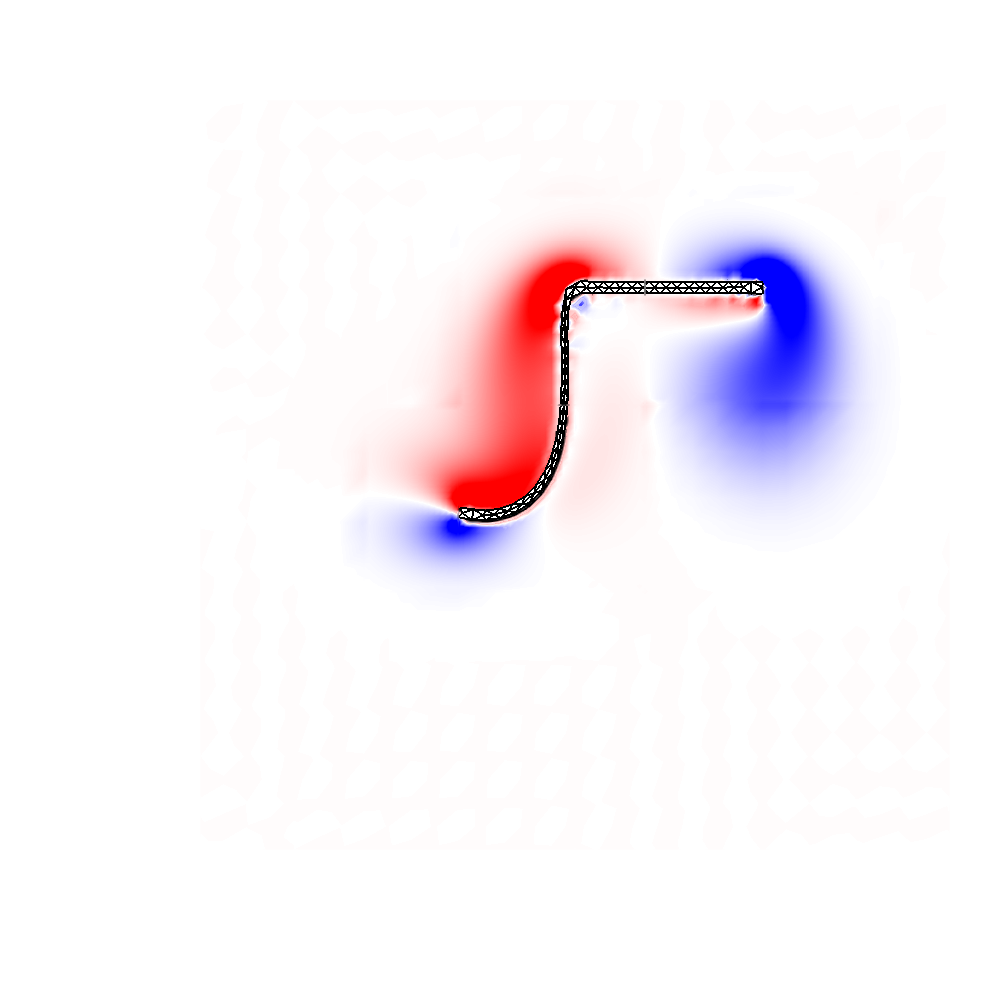
\includegraphics[width=0.88\textwidth]{ch19-half-mu1-t1.png}\\ \scriptsize $\mu = 1$, $t = 1$
\column{0.25\textwidth}\centering 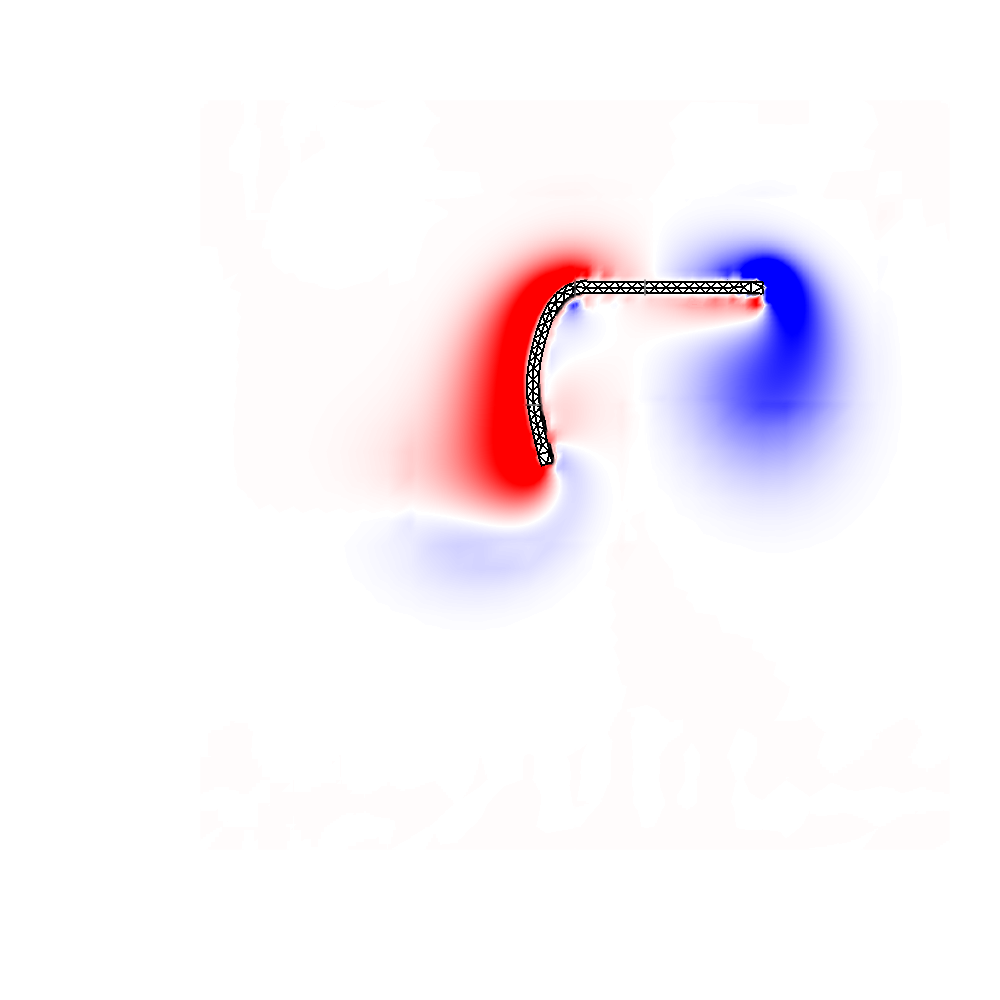
\includegraphics[width=0.88\textwidth]{ch19-half-mu10-t1.png}\\ \scriptsize $\mu = 10$ (shipped), $t = 1$
\column{0.25\textwidth}\centering 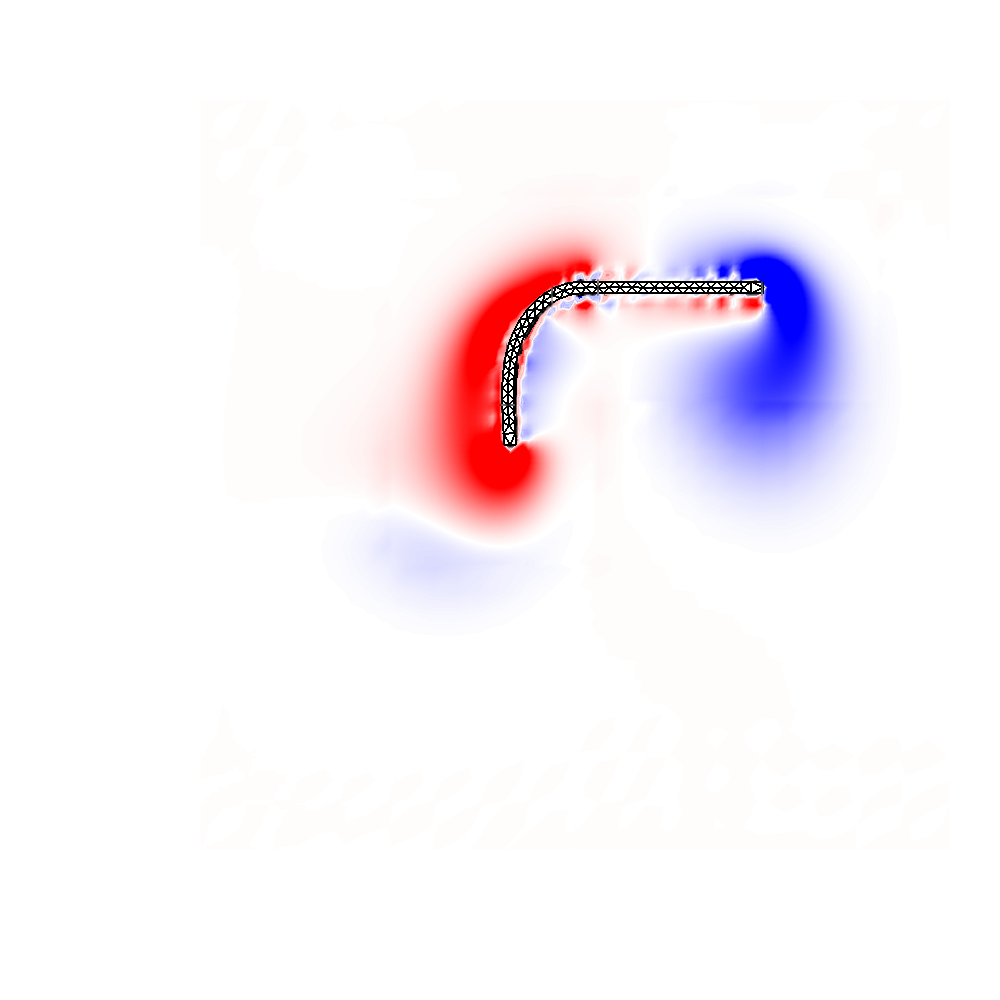
\includegraphics[width=0.88\textwidth]{ch19-half-mu100-t1.png}\\ \scriptsize $\mu = 100$, $t = 1$
\column{0.25\textwidth}\centering 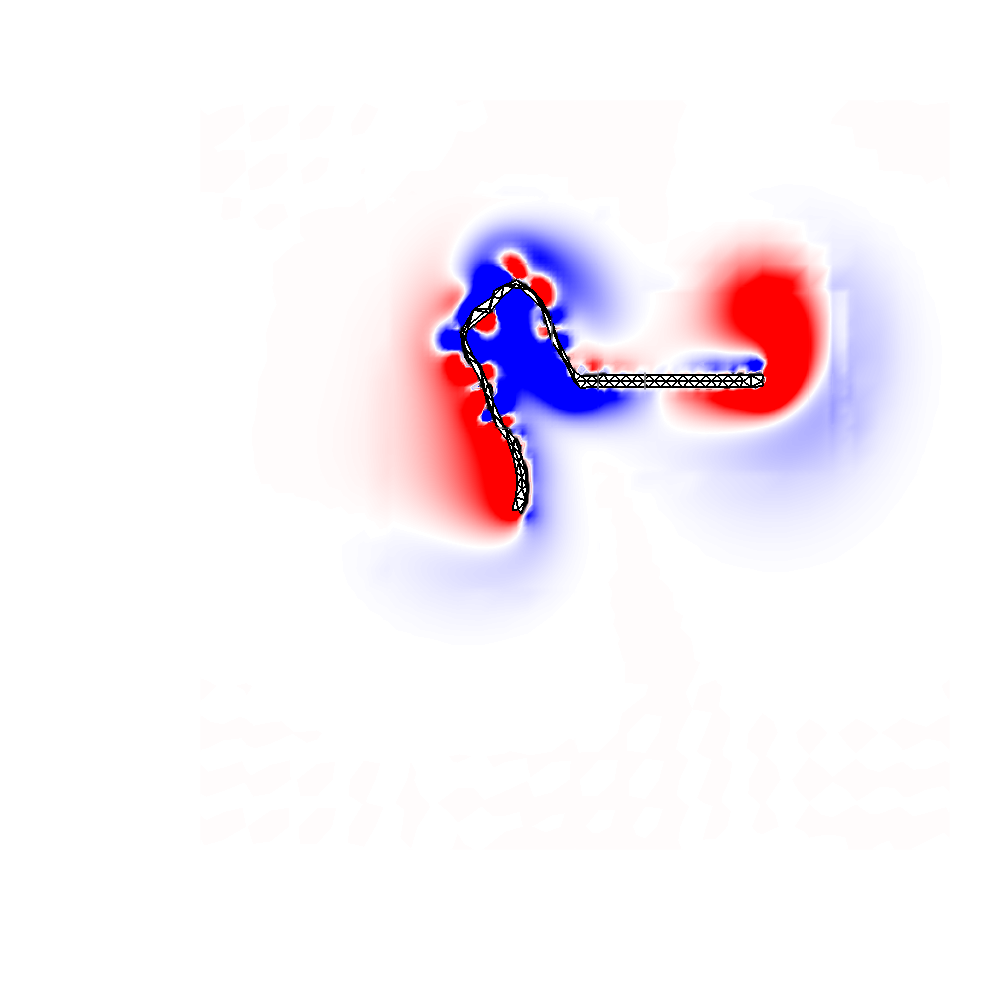
\includegraphics[width=0.88\textwidth]{ch19-half-mu1-t15.png}\\ \scriptsize $\mu = 1$, $t = 1.5$: crumpled
\end{columns}
\scriptsize
\begin{itemize}
  \item IBFE/01 with \code{MOTION = "HALF"}: the right half is pulled up at $0.5$ for one second, the left half is carried by the material law alone. Vorticity $\pm 5$, the mesh displaced by \code{dX}.
  \item $\mu = 100$: the free half follows almost rigidly, the plate tilts by about $32^\circ$. $\mu = 10$: about $39^\circ$, with a visible bend at the join. $\mu = 1$: the free half folds under the fluid's drag, its tip moves from $x = -0.5$ to about $-0.15$ by $t = 1.5$, the folding plate stirs up fast flow, and the run stops near $t = 1.6$ with \code{Time step size change encountered}; halving \code{DT} only delays it to $t \approx 2.05$ (chapter 16).
  \item A factor of ten in $\mu$ is a factor of ten in the restoring force for the same strain; the drag on the free half is fixed by the motion, so the strain scales as $1/\mu$ until it is no longer small. Chapter 8b's non-dimensional stiffness: $\mu/(\rho U^2)$ with $U = 0.5$ and $\rho = 1$ is $4$, $40$ and $400$ here.
\end{itemize}
\sourcecredit{Runs: \code{/root/work/0.19.0/try\_softplate\_dt} ($\mu = 1$, \code{DT = 5e-4}), \code{ibfe01\_HALF}, \code{try\_stiffplate}; IBAMR 0.19.0; \code{wsl/final/visit\_ch19.sh}.}
\end{frame}

% 14
\begin{frame}{Choosing $\mu$}
\label{fr:choosemu}
\footnotesize
\begin{itemize}
  \item \al{Units.} $\mathbb{P}$ is force per reference area (2D: per reference length), so $\mu$ has the units of a pressure (2D: force per length). In the examples' unit system ($\rho = 1$, $L = 2$, $U = 0.5$) a value is a multiple of $\rho U^2$; chapter 8b's rule applies: fix the dimensionless group, not the number.
  \item \al{From a real material:} $\mu = E/(2(1+\nu))$; soft tissue $E \sim 10^4$--$10^6$ Pa, rubber $\sim 10^6$ Pa, with $\nu \approx 0.45$--$0.5$. Convert to the simulation's units through $\rho U^2$ (a plate in water, $\rho = 1000$ kg/m$^3$, $U = 0.1$ m/s: $\rho U^2 = 10$ Pa, so $E = 10^4$ Pa is $\mu/(\rho U^2) \approx 350$).
  \item \al{From the behaviour you want:} the plate's bending stiffness goes as $\mu h^3$ per unit width ($h$ the thickness); halve $h$ and you need eight times $\mu$ for the same deflection. The IBFE/01 runs give the scale: $\mu/(\rho U^2) = 40$ bends visibly under its own motion, $4$ folds, $400$ hardly bends.
  \item \al{The cost of stiffness:} the explicit coupling limits the time step by the elastic wave speed, $\Delta t \lesssim \mathrm{DX}/\sqrt{\mu/\rho}$ up to a constant; $\mu = 100$ ran at \code{DT = 1e-3} ($\sqrt{\mu/\rho}\,\Delta t/\mathrm{DX} = 0.64$), and the stiff-tether chapter 9a rule ``stiffness against \code{DT}'' holds here too. A plate that must not bend at all is better tethered (chapter 17) than made stiff.
  \item \al{The cost of softness:} large strains, elements that fold, and a run that ends in \code{Time step size change encountered} when the folding body drives the fluid past the CFL limit.
\end{itemize}
\begin{punchbox}
\footnotesize Start from the example's $\mu$, predict the change you expect from $\mu/(\rho U^2)$, run, and compare with the measured tilt: chapter 8a's procedure, which is why chapter 17 recorded the numbers.
\end{punchbox}
\end{frame}

% 15
\begin{frame}[fragile]{Body forces: the signature, the tether, and the 2014 remark about $\mathbf{F}$}
\label{fr:bodyforce}
\scriptsize
``Similar to PK1 stress, you are applying a generalized force directly on the element. This is a lot easier than in the fiber version of IBAMR because you can use positional information from the reference configuration, $\mathbf{s}$. Also, because it is generalized, the forcing function can be anything of your choosing'' (2014). A body force is a vector per unit reference volume (2D: area), returned in \code{F}, from the same nine arguments:
\begin{lstlisting}[style=cpptiny]
void body_force_function(VectorValue<double>& F, const TensorValue<double>& FF, const libMesh::Point& X, const libMesh::Point& s,
                         Elem* const elem, const std::vector<const std::vector<double>*>& var_data,
                         const std::vector<const std::vector<VectorValue<double> >*>& grad_var_data, double time, void* ctx);
\end{lstlisting}
The 2014 and 2020 target-point force (chapter 17's tether, in the course's spelling):
\begin{lstlisting}[style=cpptiny]
{  libMesh::Point s_dump;
   kappa_s=1e6; //Stiffness constant
    if(time<1)      { s_dump(1)=s(1)+.5*time; s_dump(0)=s(0); }      // up at 0.5 for 0 < t < 1
    else if(time<3) { s_dump(1)=s(1)+.5+.5*(1-time); s_dump(0)=s(0); }
    else            { s_dump(1)=X(1); s_dump(0)=X(0); }              // X(.): current configuration: no force
    F = kappa_s*(s_dump-X);      //usual target point movement
    return;
}
\end{lstlisting}
\begin{itemize}
  \item ``Note that for our body force function, we want to update $\mathbf{F}$ at the end of our function'' (2014): \code{F} is the output argument; whatever it holds when the function returns is the force. Set it on every path (the \code{s\_dump = X} branch gives zero; \code{F.zero()} is the explicit form).
  \item $\kappa_s$ multiplies a displacement, so it is a stiffness per unit reference volume: force/length$^{\mathrm{NDIM}+1}$. $10^6$ in the plate's units; \code{KAPPA\_S} in the input.
\end{itemize}
\end{frame}

% 16
\begin{frame}[fragile]{Registering a body force, and the slide that got it wrong}
\label{fr:register}
\footnotesize
\begin{columns}[T]
\column{0.5\textwidth}
Correct (2014 deck, slide 12; the example):
\begin{lstlisting}[style=cpptiny]
IBFEMethod::LagBodyForceFcnData body_force_data(body_force_function);
// the second argument is the part (default 0)
ib_method_ops->registerLagBodyForceFunction(body_force_data, 0);
\end{lstlisting}
\column{0.48\textwidth}
Wrong (2020 deck, slide 12, under the heading ``Registering your Body Force''):
\begin{lstlisting}[style=cpptiny]
IBFEMethod::PK1StressFcnData active_stress_data(active_stress_function);
ib_method_ops->registerPK1StressFunction(active_stress_data);
\end{lstlisting}
\end{columns}
\end{frame}

% 16b
\begin{frame}{Registering a body force (2): what went wrong, and the counting rules}
\label{fr:register2}
\footnotesize
\begin{itemize}
  \item The 2020 slide pasted the active-\emph{stress} registration (chapter 20) under the body-force heading. A body force returns a \code{VectorValue}; a stress returns a \code{TensorValue}; the two \code{*FcnData} types take different function pointers, so putting a body force into \code{PK1StressFcnData} does not compile. Nobody could have run it, which is how it survived four years.
  \item \al{One body force function per part} (a second \code{registerLagBodyForceFunction} replaces the first); any number of stress functions; one surface force and one surface pressure per part (chapter 17, slide 25). A plate with a tether \emph{and} gravity needs both in one function.
  \item The second argument is the part: ex7 registers \code{lower\_tether\_force\_data} on part 0 and \code{upper\_tether\_force\_data} on part 1.
  \item ``When done remember to register your equation system'' (2014 slide 13): \code{initializeFEEquationSystems()} after the registrations, then \code{getFEDataManager(part)->getEquationSystems()} for the writer; chapter 17, slide 23.
\end{itemize}
\end{frame}

% 17
\begin{frame}[fragile]{Body forces (2): gravity, and anything else ``of your choosing''}
\label{fr:gravity}
\footnotesize
A body that is heavier than the fluid: gravity minus buoyancy, per unit reference volume, on every point:
\begin{lstlisting}[style=cpptiny]
static double rho_s = 1.2, rho_f = 1.0, g = 9.81;      // from the input: RHO_S, RHO (and g in the simulation's units)
void gravity_force_function(VectorValue<double>& F, const TensorValue<double>& /*FF*/, const libMesh::Point& /*X*/,
                            const libMesh::Point& /*s*/, Elem* const /*elem*/,
                            const std::vector<const std::vector<double>*>& /*var_data*/,
                            const std::vector<const std::vector<VectorValue<double> >*>& /*grad_var_data*/,
                            double /*time*/, void* /*ctx*/)
{
    F.zero();
    F(1) = -(rho_s - rho_f) * g;     // down; the fluid's own weight is in the pressure already
}
\end{lstlisting}
\begin{itemize}
  \item The IBFE solid has the fluid's density (it \emph{is} fluid, constrained to move elastically): a body force $(\rho_s - \rho_f)\mathbf{g}$ is how excess weight enters, the counterpart of chapter 13's point masses. Buoyancy is already in the fluid's hydrostatic pressure, hence the difference.
  \item A tether plus gravity: add the two terms in one function. A force that switches with time: test \code{time}, as the tether does. A force on part of the body: test \code{s}, as IBFE/10's band does (\code{|s(2)| < 0.1}). A force that depends on the deformation: use \code{FF} (a damper proportional to the rate needs the velocity, next slide).
  \item Chapter 20's active tension is \emph{not} a body force but a stress: it acts along fibres and is integrated by parts like $\mathbb{P}$. The theory repository's 4.3 has both: ``Localized tether as an external body force'' and ``Passive and active stress''.
\end{itemize}
\end{frame}

% 18
\begin{frame}[fragile]{Reading a field from the mesh: \code{system\_data}, and a damped tether (upstream ex5)}
\label{fr:sysdata}
\footnotesize
\code{var\_data} and \code{grad\_var\_data} are empty unless you ask for systems. Upstream \code{IBFE/explicit/ex5} asks for the velocity so that its tether can damp:
\begin{lstlisting}[style=cpptiny]
struct TetherData { double kappa_s_body, eta_s_body, kappa_s_surface, eta_s_surface; TetherData(Pointer<Database> input_db) {...} };
void tether_force_function(VectorValue<double>& F, const TensorValue<double>& /*FF*/, const libMesh::Point& x, const libMesh::Point& X,
                           Elem* const /*elem*/, const vector<const vector<double>*>& var_data,
                           const vector<const vector<VectorValue<double>>*>& /*grad_var_data*/, double /*time*/, void* ctx)
{
    const TetherData* const tether_data = reinterpret_cast<TetherData*>(ctx);
    const std::vector<double>& U = *var_data[0];                         // the velocity at this quadrature point
    for (unsigned int d = 0; d < NDIM; ++d)
        F(d) = tether_data->kappa_s_body * (X(d) - x(d)) - tether_data->eta_s_body * U[d];   // spring minus damper
}
...
std::vector<int> vars(NDIM); for (unsigned int d = 0; d < NDIM; ++d) vars[d] = d;
vector<SystemData> sys_data(1, SystemData(IBFEMethod::VELOCITY_SYSTEM_NAME, vars));
IBFEMethod::LagBodyForceFcnData body_fcn_data(tether_force_function, sys_data, &tether_data);
ib_method_ops->registerLagBodyForceFunction(body_fcn_data);
\end{lstlisting}
\end{frame}

% 22b
\begin{frame}{Reading a field from the mesh (2): what \code{SystemData} and \code{ctx} do}
\label{fr:sysdata2}
\footnotesize
\begin{itemize}
  \item \code{SystemData(system\_name, vars, grad\_vars)} names a libMesh system on the mesh and which of its variables you want; IBAMR evaluates them at each quadrature point and hands them over as \code{var\_data[i]} (values) and \code{grad\_var\_data[i]} (gradients), in the order you listed. \code{IBFEMethod::VELOCITY\_SYSTEM\_NAME} is the structure's velocity; \code{COORDS\_SYSTEM\_NAME} its position; chapter 20 adds a system of its own for the fibre direction.
  \item \code{ctx} carries your parameters without globals: a pointer to any struct, cast back inside. The course used \code{static} variables in \code{ModelData}; both work, \code{ctx} scales to several parts with different constants.
  \item Note the naming: ex5 follows IBAMR's headers (\code{x} current, \code{X} reference), the reverse of the course's.
\end{itemize}
\end{frame}

% 19
\begin{frame}[fragile]{Surface forces: a traction on chosen sides (upstream ex8)}
\label{fr:surface}
\footnotesize
\begin{lstlisting}[style=cpptiny]
static double beam_kappa_s = 1.0e6;
void beam_tether_force_function(VectorValue<double>& F,
                                const VectorValue<double>& /*n*/, const VectorValue<double>& /*N*/,
                                const TensorValue<double>& /*FF*/,
                                const libMesh::Point& X, const libMesh::Point& s,
                                Elem* const /*elem*/, const unsigned short int side,
                                const vector<const vector<double>*>& /*var_data*/,
                                const vector<const vector<VectorValue<double>>*>& /*grad_var_data*/,
                                double /*time*/, void* /*ctx*/)
{
    if (side == 1 || side == 3)             // the two long sides of the beam's quadrilaterals
    {
        F = beam_kappa_s * (s - X);         // a tether applied on the surface, per unit reference area
    }
    else
    {
        F.zero();
    }
}
...
// part 2 of three
ib_method_ops->registerLagSurfaceForceFunction(beam_tether_force_data, 2);
\end{lstlisting}
\end{frame}

% 23b
\begin{frame}{Surface forces (2): sides, units, and where they are used}
\label{fr:surface2}
\footnotesize
\begin{itemize}
  \item Twelve arguments (chapter 17, slide 26): the nine plus the current and reference normals \code{n}, \code{N} and the element's \code{side}. libMesh numbers a quadrilateral's sides $0$--$3$ counter-clockwise from the bottom edge and a triangle's $0$--$2$; \code{side} lets one function act on the long edges only.
  \item A surface force is per unit reference area of the boundary; it enters the weak form as $\int \mathbf{F}\phi_k\,dA$ on the boundary, alongside the traction $\mathbb{P}\mathbf{N}$. Upstream ex5 registers the \emph{same} damped tether as a body force on the interior and as a surface force on the boundary of a thin shell; the immersed-interface examples (\code{IIM/ex0}--\code{ex6}) use surface forces for everything.
  \item A surface \emph{pressure} (scalar; force $-p\,\mathbf{n}$) is the special case for loads normal to the surface: chapter 17, slide 27.
\end{itemize}
\end{frame}

% 20
\begin{frame}{What the tether stiffness does: the full plate with $\kappa_s = 10^4$}
\label{fr:kappa}
\begin{columns}[T]
\column{0.34\textwidth}
\begin{center}
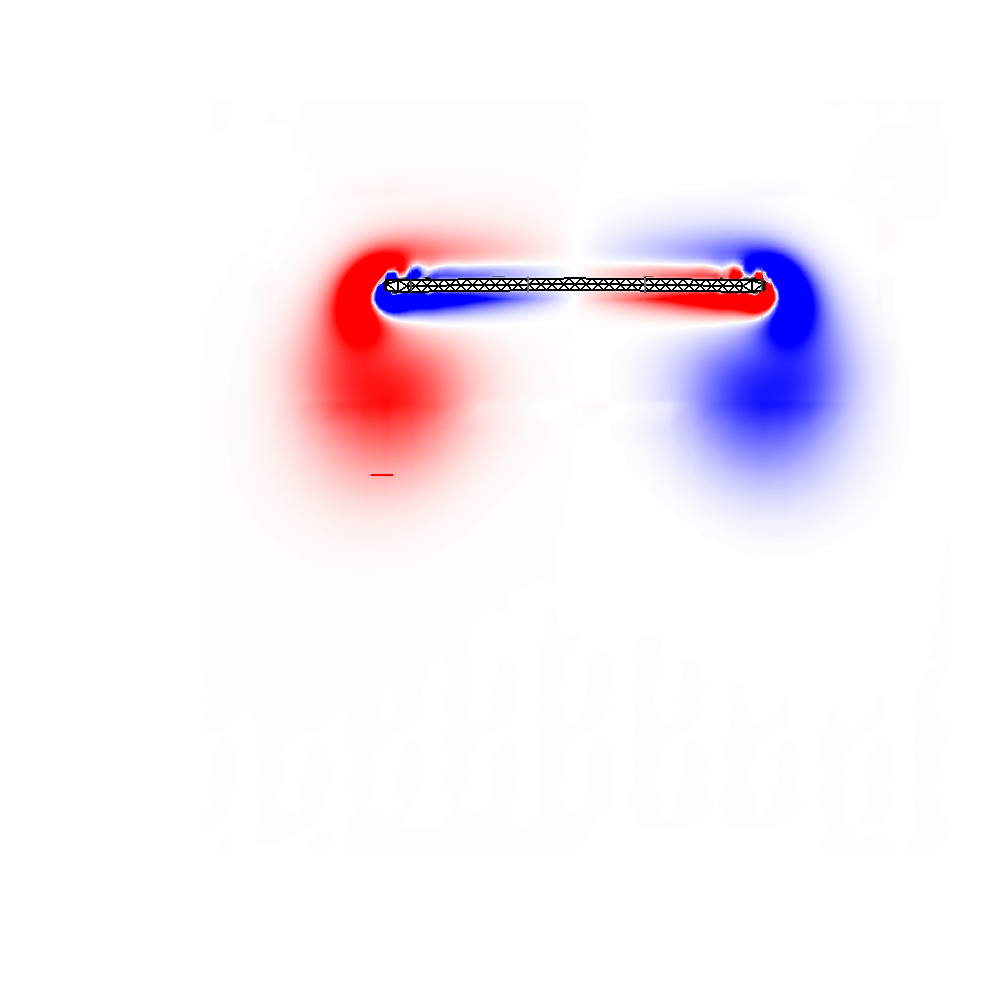
\includegraphics[width=\textwidth]{ch19-full-kappa1e4-t1.png}\\ \scriptsize $\kappa_s = 10^4$, $t = 1$
\end{center}
\column{0.64\textwidth}
\footnotesize
\begin{itemize}
  \item With the shipped $\kappa_s = 10^6$ the plate's centre is at $y = 0.500$ at $t = 1$, the target's position to three digits (chapter 17, slide 38).
  \item With $\kappa_s = 10^4$ it trails: $y = 0.241$ instead of $0.250$ at $t = 0.5$, a lag of $0.009$, and when the target turns around at $t = 1$ the plate overshoots to $0.507$. The lag is the drag divided by $\kappa_s$ times the plate's area: a hundred times softer, a hundred times the lag ($10^{-4}$ at $10^6$).
  \item At $10^2$ the plate would lag by about $1$, its own length: it no longer follows at all, and the run becomes ``a plate in a fluid with a weak spring''. Chapter 9a's rule for target points, $\kappa$ large enough that the lag is below the grid spacing, is the same rule: $\kappa_s \gtrsim F_{\mathrm{drag}}/(A\,\mathrm{DX})$.
  \item The stiffness-against-\code{DT} rule also carries over: $\kappa_s = 10^6$ at \code{DT = 1e-3} is near the limit for this grid (a stiffer tether at the same step stops with the chapter 16 error).
\end{itemize}
\end{columns}
\sourcecredit{Run: \code{/root/work/0.19.0/try\_softtether} (\code{MOTION = "FULL"}, \code{KAPPA\_S = 1.0e4}), IBAMR 0.19.0.}
\end{frame}

% 21
\begin{frame}{What can go wrong}
\label{fr:wrong}
\scriptsize
\begin{tabular}{@{}L{0.40\textwidth}L{0.52\textwidth}@{}}
\toprule
symptom & cause and fix \\
\midrule
\code{no matching function for call to ... PK1StressFcnData(void (\&)(...))} or \code{LagBodyForceFcnData(...)} & the function's signature is not the nine-argument one (a 2014 seven-argument function; a body force given to a stress struct, as on the 2020 slide); fix the arguments, use the matching struct \\
the plate shrinks or pulls in from $t = 0$ & the dilational part $-\mu\mathbb{F}^{-T}$ is missing or has the wrong sign; the reference state must give $\mathbb{P} = 0$ \\
the body has no stiffness, folds at once & the deviatoric part is missing; or $\mu$ is in the wrong units (slide \ref{fr:choosemu}) \\
\code{nan} in the log, then an abort & $\ln J$ of $J \le 0$: an inverted element (chapter 18's orientation rule), or a crumpled one (too soft, or a step too large) \\
\code{Time step size change encountered} & the body is too soft for its motion (folding drives the flow past CFL), or too stiff for \code{DT}; chapter 16 \\
the tether does not hold & $\kappa_s$ too small for the drag (slide \ref{fr:kappa}); or the force was set on one branch only (``update \code{F} at the end'') \\
the force acts on the wrong part & the part argument of \code{register*} (default $0$); or \code{s} tested in the wrong coordinate (\code{s(1)} is $y$) \\
a second body force silently replaces the first & one body force per part: combine them in one function \\
the run is slow in the structure step & work inside the stress function: allocation, I/O, or \code{std::pow} on every call; precompute, use \code{ctx} \\
\code{var\_data[0]} is empty or out of range & no \code{SystemData} given to the \code{*FcnData}, or fewer systems than you index \\
\bottomrule
\end{tabular}

\end{frame}

% 22
\begin{frame}{What the older decks had that is now Part X}
\label{fr:legacy}
\footnotesize
\begin{tabular}{@{}L{0.46\textwidth}L{0.46\textwidth}@{}}
\toprule
2014--2020 & now \\
\midrule
seven-argument callbacks with \code{const vector<NumericVector<double>*>\& system\_data} & nine arguments with \code{var\_data} and \code{grad\_var\_data} (slide \ref{fr:signature}) \\
\code{Utility::string\_to\_enum<}\newline\code{libMeshEnums::Order>} & \code{libMesh::Order} \\
``\code{-mu*F\^{}-T} enforces the incompressibility condition'' (2014, 2018, 2020) & it makes the reference state stress-free; the fluid keeps the volume (slide \ref{fr:dil}) \\
2020 slide 12: a body force registered with \code{PK1StressFcnData} & \code{LagBodyForceFcnData} + \code{registerLagBodyForceFunction} (slide \ref{fr:register}) \\
``\code{Example\_IBFE\_TargetPoints2D}'' & IBFE/01 (the example named in 2014 never shipped under that name) \\
\code{static double mu = 100} on the slides, $10$ in the examples & \code{SHEAR\_MODULUS} in the input; both values run (slide \ref{fr:mu}) \\
the 2018 overview's four equation images & the theory repository's chapters 4.1--4.3 (own derivations, own figures) \\
\bottomrule
\end{tabular}

\end{frame}

% 23
\begin{frame}{Exercises}
\label{fr:exercises}
\footnotesize
\begin{enumerate}
  \item Remove the dilational function from IBFE/01 (comment out its \code{registerPK1StressFunction}) and run \code{FULL} to $t = 0.5$. Measure the plate's length from \code{output.ex2} and explain the sign of the change from slide \ref{fr:dil}.
  \item Replace the neo-Hookean pair by the compressible law of IBFE/10 with $\beta = 10\mu$ and $\beta = 100\mu$ (\code{MOTION = "HALF"}). Print $J$'s range every 50 steps as IBFE/10 does. Which $\beta$ is worth its time step?
  \item Write the St.\ Venant--Kirchhoff law of ex7 for the plate with $\lambda = \mu$ and compare the tilt at $t = 1$ with the neo-Hookean $39^\circ$.
  \item Make the plate's left half ten times stiffer than its right (test \code{s(0)} in both stress functions), run \code{HALF}, and explain the tilt you get from slide \ref{fr:mu}.
  \item Add gravity (slide \ref{fr:gravity}) with $\rho_s - \rho_f = 0.2$ and $g = 1$ to \code{MOTION = "FULL"} after the release; where is the centre at $t = 4$ compared with chapter 17's $-0.936$?
  \item Make the tether of IBFE/01 a damped one as in ex5 ($\eta_s = 10^3$): register the velocity system, read it from \code{var\_data}, and compare the overshoot at $t = 1$ with slide \ref{fr:kappa}'s $0.507$.
  \item Turn the plate's tether into a surface force on its long edges only (ex8's \code{side} test). Does the plate still follow the target, and what does its mesh look like at $t = 1$?
\end{enumerate}
\end{frame}

% 24
\begin{frame}{Rules of thumb}
\label{fr:thumb}
\small
\begin{itemize}
  \item A stress function returns $\mathbb{P}(\mathbb{F})$ and is called at every quadrature point every step: arithmetic only.
  \item Two parts for the neo-Hookean law, $\mu\mathbb{F}$ and $-\mu\mathbb{F}^{-T}$; the second makes the reference state stress-free, the fluid keeps the volume.
  \item Register stresses as many as you like, one body force per part, one surface force and one surface pressure per part; a body force is a \code{LagBodyForceFcnData}, never a \code{PK1StressFcnData}.
  \item $\mu/(\rho U^2)$: $4$ folds, $40$ bends, $400$ barely moves, for a plate driven at $U$. Stiffer costs time step.
  \item $\kappa_s$: lag $= F_{\mathrm{drag}}/(\kappa_s A)$; keep it below a grid cell.
  \item Set \code{F} on every path; test \code{s} (reference position) for ``which part'', \code{time} for ``when'', \code{FF} for ``how much''.
  \item Want the velocity or another field inside a function: \code{SystemData} in the \code{*FcnData}, read \code{var\_data[i]}.
  \item Constants from the input, into \code{ModelData} statics or a \code{ctx} struct, before \code{initializeFEEquationSystems()}.
\end{itemize}
\end{frame}

% 25
\begin{frame}{Summary}
\label{fr:summary}
\footnotesize
\begin{enumerate}
  \item The structure's elasticity is one or more C++ functions returning the first Piola--Kirchhoff stress from the deformation gradient; IBAMR integrates $-\mathbb{P}:\nabla\phi_k$ over every element with the Gauss rule you choose, solves for nodal forces, and spreads them from quadrature points.
  \item The course's neo-Hookean model is $\mu\mathbb{F} - \mu\mathbb{F}^{-T}$ in two registered functions. The second term cancels the first in the reference state; it does not enforce incompressibility, the fluid does. The compressible variant adds $\beta\ln J$; St.\ Venant--Kirchhoff is $\mathbb{F}\mathbb{S}$ with Hooke's law in $\mathbb{E}$; all three are in the examples with their registrations.
  \item Body forces (per reference volume) and surface forces (per reference area) have the same shape as stress functions plus, for surfaces, the normals and the side; the tether is the standard body force, gravity the next, a damped tether needs the velocity through \code{SystemData}. One body force per part, registered as a body force.
  \item From runs: $\mu = 1$, $10$, $100$ fold, bend and hold the half-tethered plate; $\kappa_s = 10^4$ lags and overshoots where $10^6$ follows. Both knobs trade fidelity against the time step.
  \item The 2014 deck was right about registration and wrong about incompressibility; the 2020 deck inherited the second and added a registration that does not compile. Both are corrected here, with the theory left to the theory repository.
\end{enumerate}
\begin{homebox}
\footnotesize Chapter 20 adds the active fibre stress $J\,T\,\mathbb{F}\,\mathbf{f}_0\otimes\mathbf{f}_0$ and runs the course's three fibre-tension examples (IBFE/06).
\end{homebox}
\end{frame}

% 26
\begin{frame}{Recordings (listed, not incorporated)}
\label{fr:videos}
\small The 2020 Zoom recordings of the IBFE lectures (\emph{Apply Active Tension}, which covered this chapter and the next) are listed in the front matter's video list (chapter 0.1). Nothing in them is reproduced here.
\end{frame}

% 27
\begin{frame}{References and credits}
\label{fr:refs}
\scriptsize
\begin{itemize}
  \item B. E. Griffith and X. Luo, \emph{Hybrid finite difference/finite element immersed boundary method}, Int.\ J.\ Numer.\ Meth.\ Biomed.\ Eng.\ 33 (2017) e2888 (the weak form, the quadrature-point spreading, the stress splitting).
  \item J. Bonet and R. D. Wood, \emph{Nonlinear Continuum Mechanics for Finite Element Analysis}, 2nd ed., Cambridge University Press, 2008 (the 2014 deck's book link). G. A. Holzapfel, \emph{Nonlinear Solid Mechanics}, Wiley, 2000 (hyperelastic laws for tissue).
  \item The theory repository: \emph{Fluid Dynamics and IBM Theory}, chapters 4.1 \emph{The mechanics, coupling and tradeoffs of IBFE} (30 slides), 4.2 \emph{Kinematics, strain, stress and hyperelasticity} (83), 4.3 \emph{Strong form, weak form and discrete coupling} (40). \url{https://github.com/fairyflies9/Fluid-Dynamics-and-IBM-Theory}
  \item IBAMR 0.19.0: \code{src/IB/FEMechanicsBase.cpp} (the force assembly and the registration functions), \code{include/ibamr/FEMechanicsBase.h}, \code{ibtk/include/ibtk/libmesh\_utilities.h} (\code{SystemData}, \code{tensor\_inverse\_transpose}, \code{outer\_product}); \code{examples/IBFE/explicit/ex2}, \code{ex4}, \code{ex5}, \code{ex7}, \code{ex8}. \url{https://github.com/IBAMR/IBAMR}
  \item The examples of this series: IBFE/01 (the runs of slides \ref{fr:mu} and \ref{fr:kappa}), IBFE/10 (the compressible law); \code{wsl/final/visit\_ch19.sh}.
  \item Sources: Alex Hoover, \emph{3-IBFE Tutorial: PK1 Stress and Body Forces} (UNC, 2014, edited 2016); \emph{4-IBFE Lecture: Apply Active Tension}, slides 1--14 (2020; ``adapted from Alex Hoover''); \emph{2-IBFE Method: General Overview} (2018).
\end{itemize}
\end{frame}

\end{document}
